%! Author = Nhan Huynh
%! Date = 17/01/2022

% Preamble
\documentclass{../tuda-beamer}

% Tikz
\usetikzlibrary{mindmap}

% Title information
\authors{Simon Hock}
\authors{Nhan Huynh}
\authors{Daniel Mangold}
\date{19. Januar 2022}

% Document
\begin{document}
    \maketitle

    \begin{frame}{Überblick}
        \tableofcontents
    \end{frame}


    \section{Generics [5min]}
    \label{sec:generics}
    \begin{frame}[c]{Generics}
        \begin{itemize}
            \item Generizität nur auf \textbf{Referenztypen} möglich!
            \item Abstraktion, Wiederverwendbarkeit von Klassen bzw. Methoden
            \item Weniger redundanter Code, da man eine Klasse/ Methode durch Generizität auf
            mehrere Referenztypen anwenden kann, ohne diese speziell für einen Typ zu spezifizieren.
        \end{itemize}
    \end{frame}


    \section{Kovarianz [10min]}
    \label{sec:kovarianz}
    \begin{frame}[c]{Kovarianz }
        \begin{itemize}
            \item Beruhen auf dem Ersetzbarkeitsprinzip
            \item Der zurückgelieferte Wert der Unterklassen muss mit dem der Oberklasse
            vereinbar sein, also es darf kein allgemeinerer Typ sein
            \item Wo kann das auftreten?
            \begin{itemize}
                \item Parameter
                \item Rückgabetyp
                \item \inlinejava{throws}-klausel
            \end{itemize}
        \end{itemize}
    \end{frame}

    \subsection{Rückgabewert}
    \label{subsec:kovarianz-rückgabewert}
    \begin{frame}[c]{Rückgabewert}
        \begin{itemize}
            \item Der aktuale Rückgabetyp entspricht entweder dem formalen Rückgabetyp oder ist
            ein Subtyp vom formalen Rückgabetyp
            \begin{itemize}
                \item Rückgatetyp \(\neq\) Rückgabewert
            \end{itemize}
        \end{itemize}

        \begin{note}[title=Rückblick:]
            \begin{itemize}
                \item \emph{Statischer Typ}:
                \begin{itemize}
                    \item Typ, der bei der Variablendeklaration angegeben wird
                    \item Ist bei der Kompilierung bekannt
                \end{itemize}
                \item \emph{Dynamischer Typ}:
                \begin{itemize}
                    \item Typ des tatsächlichen Objekts
                    \item Ist erst zur Laufzeit bekannt
                    \item Kann vom statischen Typ abweichen \(\rightarrow\) Gleich oder Subtyp des statischen
                    Typs
                \end{itemize}
            \end{itemize}
        \end{note}
    \end{frame}

    \begin{frame}[c]{Beispiel}
        \lstinputlisting[style=Java, label={lst:number-adder}]{codes/NumberAdder.java}
    \end{frame}

    \begin{frame}[c]
        \lstinputlisting[
            style=Java,
            label={lst:adder-implementation}
        ]{codes/AdderImplementation.java}
    \end{frame}

    \begin{frame}[c]
        \begin{enumerate}
            \item Welchen Typ hat die Zeile 7?
            \item Welchen Typ hat die Zeile 8?
        \end{enumerate}
        \lstinputlisting[
            style=Java,
            label={lst:number-adder-example}
        ]{codes/NumberAdder_Example.java}

        \pause
        \begin{enumerate}
            \item \inlinejava{Number}
            \item \inlinejava{Integer}
        \end{enumerate}
    \end{frame}

    \subsection{Arrays}
    \label{subsec:arrays}
    \begin{frame}[c]{Arrays}
        \begin{itemize}
            \item Die Komponententypen im Array können gleich dem Komponententypen oder ein
            Subtyp dessen sein
            \item Der dynamische Typ des Arrays kann gleich dem statischen Typ oder ein Subtyp
            dessen sein
        \end{itemize}

        \begin{figure}[h]
            \centering
            \begin{memory}[scale=.725]
                \allocatedummy{5}
                \allocatedummy{15}
                \allocatedummy{25}
                \allocate{8}{12}
                \allocate{18}{18}
                \assign{23}{18}{\inlinejava{a}}
                \assign{2}{8}{\inlinejava{a[0]} \(\leftarrow\) (Kann ein Subtyp sein)}
                \assign{8}{10}{\dots}
                \assign{14}{11}{\inlinejava{a[3]}}
                \assign{16}{12}{\inlinejava{a[4]}}
                \assignblock{18}{8}
            \end{memory}
            \caption{Abstrakte Visualisierung des Speicherplatzes eines Arrays \inlinejava{a}}
            \label{fig:array}
        \end{figure}
    \end{frame}

    \begin{frame}[c]{Beispiel: Komponententypen}
        \lstinputlisting[
            style=Java,
            label={lst:array-components-subtype}
        ]{codes/Array_Components_Subtype.java}
    \end{frame}

    \begin{frame}[c]{Beispiel: Dynamischer Typ}
        \lstinputlisting[
            style=Java,
            label={lst:array-dynamic-type}
        ]{codes/Array_Dynamic_Type.java}
    \end{frame}

    \begin{frame}
        Wirft die Zeile 5 einen Fehler? (Begründung)

        Wenn ja:

        \begin{enumerate}
            \item Welcher Fehler wird geworfen?
            \item Wird der Fehler während der Kompilierung oder erst zur Laufzeit erkannt?
        \end{enumerate}

        \lstinputlisting[
            style=Java,
            label={lst:array-dynamic-type-exception}
        ]{codes/Array_Dynamic_Type_Exception.java}

        \pause

        \begin{enumerate}
            \item \inlinejava{ArrayStoreException}
            \item Der Fehler wird erst zur Laufzeit erkannt, da der Komponententyp ein Subtyp des
            statischen Types des Arrays ist
        \end{enumerate}
    \end{frame}

    \begin{frame}[c]{Wildcards}
        \begin{itemize}
            \item Wie sieht es mit Wilcards aus?
            \item Die Typparameter sind fest d.h. es ist nicht erlaubt, anstelle des eigentlichen
            Typparameters jetzt andere direkt oder indirekt abgeleitete Klassen einzusetzen
            \begin{itemize}
                \item Nichtübertragbarkeit von Vererbung auf Typparameter
            \end{itemize}
            \item \enquote{Die Typparameter werden vom Compiler fest in die Klasse gebrannt}
        \end{itemize}
    \end{frame}

    \begin{frame}[c]
        \lstinputlisting[
            style=Java,
            label={lst:printer}
        ]{codes/Printer.java}
        \lstinputlisting[
            style=Java,
            label={lst:printer-examples}
        ]{codes/Printer_Examples.java}
    \end{frame}


    \section{Wildcards [10min]}
    \label{sec:wildcards}
    \begin{frame}[c]{Wildcards}
        \begin{itemize}
            \item Ermöglicht Kovarianz bei Typparametern
            \item Definition der Einschränkungen bei der \textbf{\emph{Instanziierung}} von
            Typparametern!
            \item Flexibilität von Typparamer von Objekten
            \item Sei \inlinejava{X} eine generische Klasse mit einem Typparamer \inlinejava{T}:
            \begin{itemize}
                \item Nach unten beschränkt: \inlinejava{X<}\underline{\inlinejava{? super
                T}}\inlinejava{>}-- \emph{Lower bounded Wildcard}
                \item Nach oben beschränkt: \inlinejava{X<}\underline{\inlinejava{? extends
                T}}\inlinejava{>}-- \emph{Upper bounded Wildcard}
            \end{itemize}
        \end{itemize}
    \end{frame}

    \begin{frame}[c]{Beispiel}
        \lstinputlisting[
            style=Java,
            label={lst:printer-wildcard}
        ]{codes/Printer_Wildcard.java}
    \end{frame}

    \subsection{Lower bounded Wildcard}
    \label{subsec:wildcards-lowerbound}
    \begin{frame}[c]{Lower bounded Wildcard}
        \begin{itemize}
            \item Typparameter nach unten in der Vererbungshierarchie beschränkt
            \item Typparameter ist entweder
            \begin{itemize}
                \item \inlinejava{T} oder
                \item direkt oder indirekte Oberklassen von \inlinejava{T} oder
                \item direkt oder indirekte implementierte Interfaces von \inlinejava{T}
            \end{itemize}
            \item Formaler Aufbau: \inlinejava{? super T}
        \end{itemize}
    \end{frame}

    \begin{frame}[c]{Katzenhierachie}
        \lstinputlisting[
            style=Java,
            label={lst:cat-hierarchy}
        ]{codes/Cat_Hierarchy.java}
    \end{frame}

    \begin{frame}[c]{Beispiel}
        Wir möchten eine schwarze Maine Coon Katze in einer Liste hinzufügen:

        \lstinputlisting[
            style=Java,
            label={lst:black-maine-coon-cat}
        ]{codes/BlackMaineCoonCat.java}

        \pause

        Das erlaubt uns nur das Hinzufügen einer schwarzen Maine Coon Katze in einer
        \inlinejava{List<BlackMaineCoonCat>}.
        Kann man das nicht flexibler machen?
    \end{frame}

    \begin{frame}[c]
        \lstinputlisting[
            style=Java,
            label={lst:black-maine-coon-cat-wildcard}
        ]{codes/BlackMaineCoonCat_Wildcard.java}
    \end{frame}

    \begin{frame}[c]
        \lstinputlisting[
            style=Java,
            label={lst:black-maine-coon-cat-wildcard-example}
        ]{codes/BlackMaineCoonCat_Wildcard_Example.java}
    \end{frame}

    \begin{frame}{Lesen}
        Welchen Typ können wir in der Zeile 4 lesen?

        \lstinputlisting[
            style=Java,
            label={lst:black-maine-coon-cat-wildcard-read}
        ]{codes/BlackMaineCoonCat_Wildcard_Read.java}
    \end{frame}

    \begin{frame}[c]
        \begin{figure}[h]
            \centering
            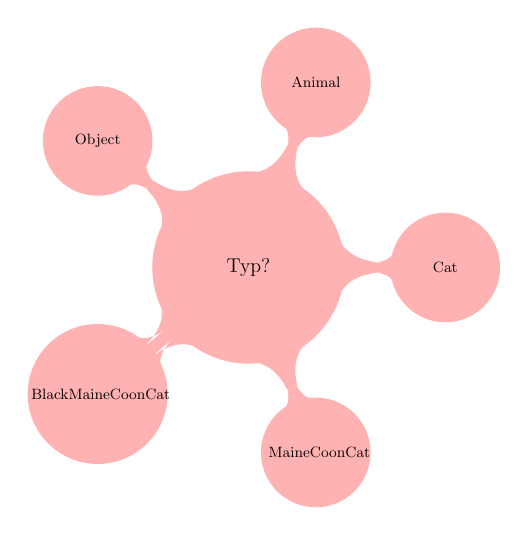
\begin{tikzpicture}[
                mindmap,
                concept color=red!30,
                every node/.style={concept, scale=0.6},
                grow cyclic,
                level 1/.append style={
                level distance=2.5cm,
                sibling angle=70,
                },
            ]
                \node {Typ?}
                child {
                    node[text width=8em] {
                        BlackMaineCoonCat
                    }
                }
                child {
                    node {
                        MaineCoonCat
                    }
                }
                child {
                    node {
                        Cat
                    }
                }
                child {
                    node {
                        Animal
                    }
                }
                child {
                    node {
                        Object
                    }
                };
            \end{tikzpicture}
            \label{fig:black-maine-coon-cat}
        \end{figure}
    \end{frame}

    \begin{frame}[c]{Welchen Typ können wir in allen Fällen garantieren?}
        Alle Klassen erben direkt oder indirekt von der Klasse \inlinejava{Object}, also können
        wir mindestens den Typ \inlinejava{Object} garantieren!

        \lstinputlisting[
            style=Java,
            label={lst:black-maine-coon-cat-wildcard-read-solution}
        ]{codes/BlackMaineCoonCat_Wildcard_Read_Solution.java}
    \end{frame}

    \begin{frame}{Schreiben}
        Welche Zeilen laufen fehlerfrei durch?

        \lstinputlisting[
            style=Java,
            label={lst:black-maine-coon-cat-wildcard-write}
        ]{codes/BlackMaineCoonCat_Wildcard_Write.java}
    \end{frame}

    \begin{frame}[c]
        Listentyp ist entweder:

        \begin{itemize}
            \item Tatsächlicher Listentyp: \inlinejava{BlackMaineCoonCat}
            \begin{itemize}
                \item Kann nur \inlinejava{BlackMaineCoonCat} oder Subtypen dessen einfügen
                \item Fehlerhafte Zeilen: 4, 5, 6,7
            \end{itemize}
            \item Tatsächlicher Listentyp: \inlinejava{MaineCoonCat}
            \begin{itemize}
                \item Kann nur \inlinejava{MaineCoonCat} oder Subtypen dessen einfügen
                \item Fehlerhafte Zeilen: 5, 6,7
            \end{itemize}
            \item Tatsächlicher Listentyp: \inlinejava{Cat}
            \begin{itemize}
                \item Kann nur \inlinejava{Cat} oder Subtypen dessen einfügen
                \item Fehlerhafte Zeilen: 6, 7
            \end{itemize}
            \item Tatsächlicher Listentyp: \inlinejava{Animal}
            \begin{itemize}
                \item Kann nur \inlinejava{Animal} oder Subtypen dessen einfügen
                \item Fehlerhafte Zeilen: 7
            \end{itemize}
            \item Tatsächlicher Listentyp: \inlinejava{Object}
            \begin{itemize}
                \item Kann nur \inlinejava{Object} oder Subtypen dessen einfügen
                \item Fehlerhafte Zeilen: Keine
            \end{itemize}
        \end{itemize}
    \end{frame}

    \begin{frame}[c]{Welchen Typ können wir in allen Fällen garantieren?}
        Wir können in jeder Liste eine \inlinejava{BlackMaineCoonCat} oder ein Subtypen dessen
        auf jeden Fall hinzufügen!

        \lstinputlisting[
            style=Java,
            label={lst:black-maine-coon-cat-wildcard-write-solution}
        ]{codes/BlackMaineCoonCat_Wildcard_Write_Solution.java}
    \end{frame}

    \subsection{Upper bounded Wildcard}
    \label{subsec:wildcards-upperbound}
    \begin{frame}[c]{Upper bounded Wildcard}
        \begin{itemize}
            \item Typparameter nach oben in der Vererbungshierarchie beschränkt.
            \item Typparameter ist entweder
            \begin{itemize}
                \item \inlinejava{T} oder
                \item direkt oder indirekte Unterklasse von \inlinejava{T} oder
            \end{itemize}
            \item Formaler Aufbau: \inlinejava{? extends T}
            \item \inlinejava{?} = \inlinejava{? extends Object}
        \end{itemize}
    \end{frame}

    \begin{frame}[c]{Beispiel}
        Wir möchten dieser Summe von Zahlen in einer Liste bilden:

        \lstinputlisting[
            style=Java,
            label={lst:sumt}
        ]{codes/Sum.java}

        \pause

        Das erlaubt uns nur dass Bilden einer Summe für den Typparameter
        \inlinejava{Number}.
        Was machen wir, wenn wir die Summe von \inlinejava{Integer} oder \inlinejava{Double}
        bilden wollen, ohne redundanten Code zu schreiben?
    \end{frame}

    \begin{frame}[c]
        \lstinputlisting[
            style=Java,
            label={lst:sum-wildcard}
        ]{codes/Sum_Wildcard.java}
    \end{frame}

    \begin{frame}[c]
        \lstinputlisting[
            style=Java,
            label={lst:sum-wildcard-example}
        ]{codes/Sum_Wildcard_Example.java}
    \end{frame}

    \begin{frame}{Lesen}
        Welchen Typ können wir in der Zeile 3 lesen? (Außerdem Number)

        \lstinputlisting[
            style=Java,
            label={lst:sum-wildcard-read}
        ]{codes/Sum_Wildcard.java}
    \end{frame}

    \begin{frame}[c]
        \begin{figure}[h]
            \centering
            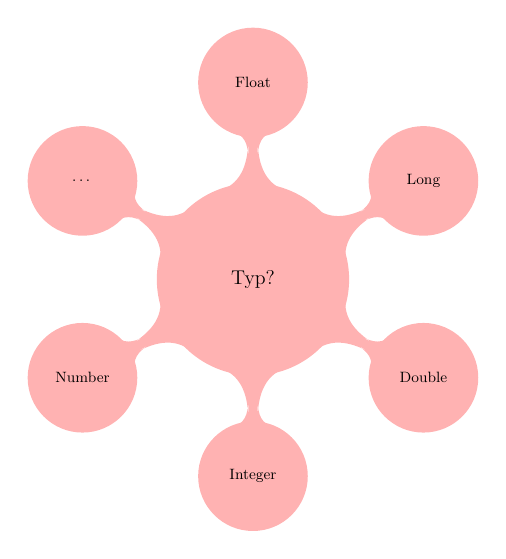
\begin{tikzpicture}[
                mindmap,
                concept color=red!30,
                every node/.style={concept, scale=0.6},
                grow cyclic,
                level 1/.append style={
                level distance=2.5cm,
                sibling angle=60,
                },
            ]
                \node {Typ?}
                child {
                    node {
                        Number
                    }
                }
                child {
                    node {
                        Integer
                    }
                }
                child {
                    node {
                        Double
                    }
                }
                child {
                    node {
                        Long
                    }
                }
                child {
                    node {
                        Float
                    }
                }
                child {
                    node {
                        \dots
                    }
                };
            \end{tikzpicture}
            \label{fig:sum}
        \end{figure}
    \end{frame}

    \begin{frame}[c]{Welchen Typ können wir in allen Fällen garantieren?}
        Alle Klassen sind Subtypen von \inlinejava{Number}, also können
        wir mindestens den Typ \inlinejava{Number} garantieren!

        \lstinputlisting[
            style=Java,
            label={lst:sum-read-solution}
        ]{codes/Sum.java}
    \end{frame}

    \begin{frame}{Schreiben}
        Welche Zeilen laufen fehlerfrei durch?

        \lstinputlisting[
            style=Java,
            label={lst:sum-wildcard-write}
        ]{codes/Sum_Wildcard_Write.java}
    \end{frame}

    \begin{frame}[c]
        Listentyp ist entweder:

        \begin{itemize}
            \item Tatsächlicher Listentyp: \inlinejava{Number}
            \begin{itemize}
                \item Kann \inlinejava{Number} oder ein Subtyp dessen einfügen
                \item Fehlerhafte Zeilen: Keine
            \end{itemize}
            \item Tatsächlicher Listentyp: \inlinejava{Integer}
            \begin{itemize}
                \item Kann \inlinejava{Integer} oder ein Subtyp dessen einfügen
                \item Fehlerhafte Zeilen: 5, 7
            \end{itemize}
            \item Tatsächlicher Listentyp: \inlinejava{Double}
            \begin{itemize}
                \item Kann \inlinejava{Double} oder ein Subtyp dessen einfügen
                \item Fehlerhafte Zeilen: 5, 6
            \end{itemize}
            \item Tatsächlicher Listentyp: \inlinejava{Long}
            \begin{itemize}
                \item Kann \inlinejava{Double} oder ein Subtyp dessen einfügen
                \item Fehlerhafte Zeilen: 5, 6, 7
            \end{itemize}
            \item \dots
        \end{itemize}
    \end{frame}

    \begin{frame}[c]{Welchen Typ können wir in allen Fällen garantieren?}
        Wir können in jeder Liste auf jeden Fall \inlinejava{null} hinzufügen!

        \lstinputlisting[
            style=Java,
            label={lst:sum-wildcard-write-solution}
        ]{codes/Sum_Wildcard_Write_Solution.java}
    \end{frame}

    \begin{frame}{Zusammenfassung}
        Gegeben sei eine Liste \inlinejava{List<E>} mit einem beliebigen Typ \inlinejava{E}.

        \begin{itemize}
            \item Schreiben erfolgt mittels der Methode \href{https://docs.oracle.com/en/java/javase/11/docs/api/java.base/java/util/List.html\#add(E)}{\inlinejava{add(E e)}}
            \item Lesen erfolgt mittels der Methode \href{https://docs.oracle.com/en/java/javase/11/docs/api/java.base/java/util/List.html\#get(int)}{\inlinejava{get(int index)}}
        \end{itemize}

        \begin{table}[h]
            \rowcolors{2}{white}{gray!25}
            \centering
            \begin{tabular}{lp{4.5cm}ll}
                \toprule
                \textbf{Statischer Typ der Liste} & \textbf{Dynamischer Typ der Liste} &
                \textbf{Schreiben} & \textbf{Lesen}
                \\
                \midrule
                \inlinejava{List<?>} & \inlinejava{Object} und alle Subklassen von
                \inlinejava{Object} & Nur \inlinejava{null} & \inlinejava{Object}
                \\
                \inlinejava{List<? super E>} & \inlinejava{E} und alle Basisklassen und
                implementierten Interfaces von \inlinejava{E} & Nur
                \inlinejava{null} & \inlinejava{T}
                \\
                \inlinejava{List<? extends E>} & \inlinejava{E} und alle Subklassen von
                \inlinejava{E} & \inlinejava{E} und alle Subtypen von \inlinejava{E} &
                \inlinejava{Object}
                \\
                \bottomrule
            \end{tabular}
            \caption{Überblick Wildcards}
            \label{tab:overview}
        \end{table}
    \end{frame}


    \section{Arbeitsphase [80min]}
    \label{sec:arbeitsphase}
    \begin{frame}[c]{Arbeitsphase}
        \begin{center}
            \textbf{\LARGE Selbstständiges Arbeiten}
        \end{center}
    \end{frame}
\end{document}
